\documentclass{article}
%encoding
%--------------------------------------
\usepackage[utf8]{inputenc}
\usepackage[T1]{fontenc}
%--------------------------------------
 
%German-specific commands
%--------------------------------------
\usepackage[ngerman]{babel}
\usepackage{csquotes}
%--------------------------------------

%Pictures
%--------------------------------------
\usepackage{graphicx}
\graphicspath{ {./Pictures/} }
\usepackage{tikz}
\usepackage{subcaption}
\usepackage{float}
\usepackage{wrapfig}
%--------------------------------------

%math
%--------------------------------------
\usepackage{amsmath}
\usepackage{amssymb}
\usepackage{amsfonts}
%--------------------------------------

%Frames
%--------------------------------------
\usepackage{framed}

%Colors
%--------------------------------------
\usepackage{xcolor}
\definecolor{blue-violet}{rgb}{0.54, 0.17, 0.89}
\definecolor{codegreen}{rgb}{0,0.6,0}
\definecolor{codegray}{rgb}{0.5,0.5,0.5}
\definecolor{codepurple}{rgb}{0.58,0,0.82}
\definecolor{backcolour}{rgb}{0.95,0.95,0.92}

%--------------------------------------
\usepackage{multicol}
\usepackage[shortlabels]{enumitem}

%Aufgaben
%--------------------------------------
\usepackage{amsthm}
\newtheorem{aufgabe}{Aufgabe}[section]
\newtheorem{definition}{Definition}[section]
\newtheorem{beispiel}{Beispiel}[section]
\newtheorem*{lernaufgabe*}{Lernaufgabe}
%--------------------------------------

%Listings
%--------------------------------------
\usepackage{ulem}
\usepackage{listings}
 
\lstdefinestyle{mystyle}{
    backgroundcolor=\color{backcolour},   
    commentstyle=\color{codegreen},
    keywordstyle=\color{magenta},
    numberstyle=\tiny\color{codegray},
    stringstyle=\color{codepurple},
    basicstyle=\ttfamily\footnotesize,
    breakatwhitespace=false,         
    breaklines=true,                 
    captionpos=b,                    
    keepspaces=true,                 
    numbers=left,                    
    numbersep=5pt,                  
    showspaces=false,                
    showstringspaces=false,
    showtabs=false,                  
    tabsize=2,
}
 
\lstset{style=mystyle,moredelim=[is][\sout]{|}{|}}
%--------------------------------------


\title{Fliesskommazahlen -- Unterrichtskonzeption}
\author{Alexandra Maximova}
\date{FS2020}

\begin{document}

\maketitle


\section*{Rahmenbedingungen}
Die LPU richtet sich an SuS, die das zweite Semester des Ergänzungsfachs Informatik absolvieren. Die SuS haben Physik und angewandte Mathematik als Schwepunktfach gewählt, und haben keine besondere Mühe mit Mathematik.

Die Fliesskommazahlen sind das zweite Thema im Modul \textbf{'Daten Darstellen'}. In diesem Modul beschäftigen wir uns grundsätzlich mit folgender Frage: Warum sagt man, dass Computer nur Nullen und Einser speichern können, wenn wir doch alle sehen, dass Computer Texte, Bilder und Videos speichern?  Diese haben doch auf dem ersten Blick gar nichts mit Nullen und Einser zu tun.

Das erste Thema des Moduls 'Daten Darstellen' waren ganze Zahlen. Die SuS haben die Zweierkomplement-Darstellung kennengelernt. Das zweite Thema, die Fliesskommazahlen, wurde schon in der vorherigen Stunde eingeführt, und die SuS haben sich schon mit der Kasten-und-Seil Metapher befasst\footnote{Diese Metapher wird genauer unten beschrieben}.

Diese LPU umfasst die zweite und dritte Stunde zum Thema Fliesskommazahlen. In der zweiten Stunde liegt der Fokus auf der Verteilung von den Fliesskommazahlen auf dem Zahlenstrahl und in der dritten Stunde wird die Addition eingeführt.

\section*{Stoffanalyse}
\begin{figure}[H]
\centering
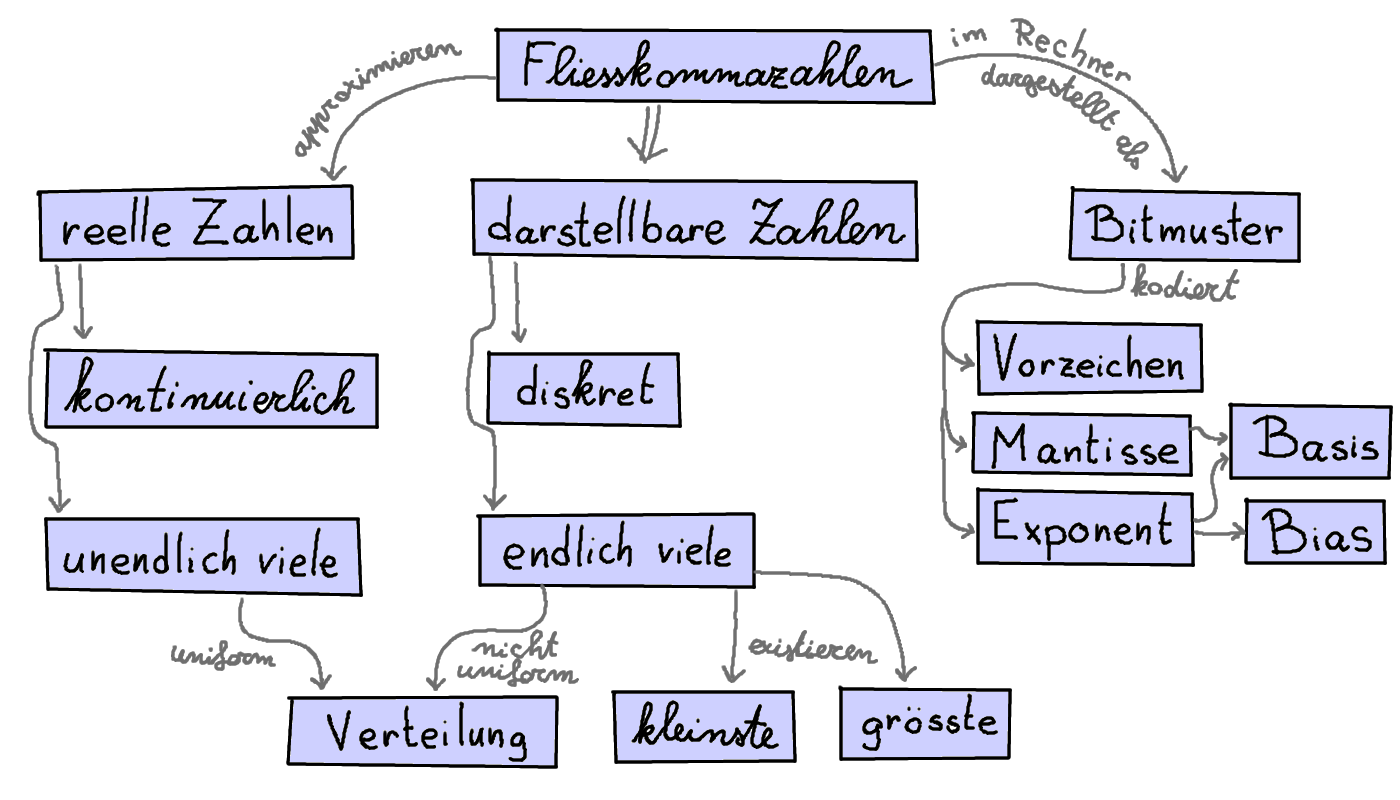
\includegraphics[width=\textwidth]{Pictures/Fliesskommazahlen_Concept_Map.png} 
\end{figure}

Die \textbf{Fliesskommazahlen} werden eingesetzt, um \textbf{reelle Zahlen} zu approximieren. Die reelle Zahlen werden in der Exponentialdarstellung in Basis 2 als \(x = (-1)^s \cdot m \cdot 2^e\) geschrieben, wobei \(s\) das \textbf{Vorzeichenbit} ist, \(m\) die \textbf{Mantisse} und \(e\) der \textbf{Exponent}. Damit die Schreibweise eindeutig ist, verlangt man \(1 \leq m < 10\).

In Computer steht für Exponent und Mantisse eine \textbf{endliche Anzahl Bits} zur Verfügung. Deswegen in einem Fliesskommazahlensystem mit fixer Mantissen- und Exponentenlänge kann man nur \textbf{endlich viele}  der \textbf{unendlich vielen} reellen Zahlen darstellen. Das bedeutet insbesondere, dass es eine \textbf{kleinste positive darstellbare Zahl}, nämlich \((-1)^0 \cdot 1.000\ldots000 \cdot 2^{e_{min}}\), und eine \textbf{grösste positive darstellbare Zahl}, nämlich \((-1)^0 \cdot 1.111\ldots111 \cdot 2^{e_{max}}\), gibt. Die Exponenten \(e_{min}\) und \(e_{max}\) sind der kleinste, bzw der grösste mögliche Exponent.

Aus der endlichen und fixen Länge von Mantisse und Exponent folgt auch, dass die Fliesskommazahlen \textbf{diskret} sind: Während zwischen zwei reellen Zahlen gibt es immer eine dritte, findet man im Fliesskommazahlensystem Zahlenpaare, zwischen denen keine darstellbare Zahl existiert.

In Gegensatz zu reellen oder ganzen Zahlen, die auf dem Zahlenstrahl \textbf{gleichmässig verteilt} sind, sind darstellbare Zahlen um die Null konzentriert\footnote{Um ganz exakt zu sein, müsste man aus dieser Beschreibung den Bereich zwischen der grössten negativen darstellbaren Zahl und der kleinsten positiven darstellbaren Zahl ausschliessen} und werden mit wachsendem Exponenten immer zerstreuter.

Im Computer werden Fliesskommazahlen als \textbf{Bitmuster} kodiert: 1 Bit wird für das Vorzeichenbit \(s\) verwendet, eine fixe Anzahl Bits für die Mantisse \(m\), wobei man das führende ''\(1.\)'' weglässt und eine fixe Anzahl Bits für den Exponenten \(e\). Die Mantisse wird eins zu eins übernommen, während der Exponent wird ''zentriert'' indem man zu \(e\) den \textbf{Bias} addiert. Der Bias hängt von der Anzahl Bits ab, die für den Exponenten reserviert sind, und wird meistens so gewählt, dass \(e = 0\) durch die Bitfolge \texttt{100...0} dargestellt wird.


\subsection*{Metapher vom Kasten und Seil}

\begin{figure}[H]
\centering
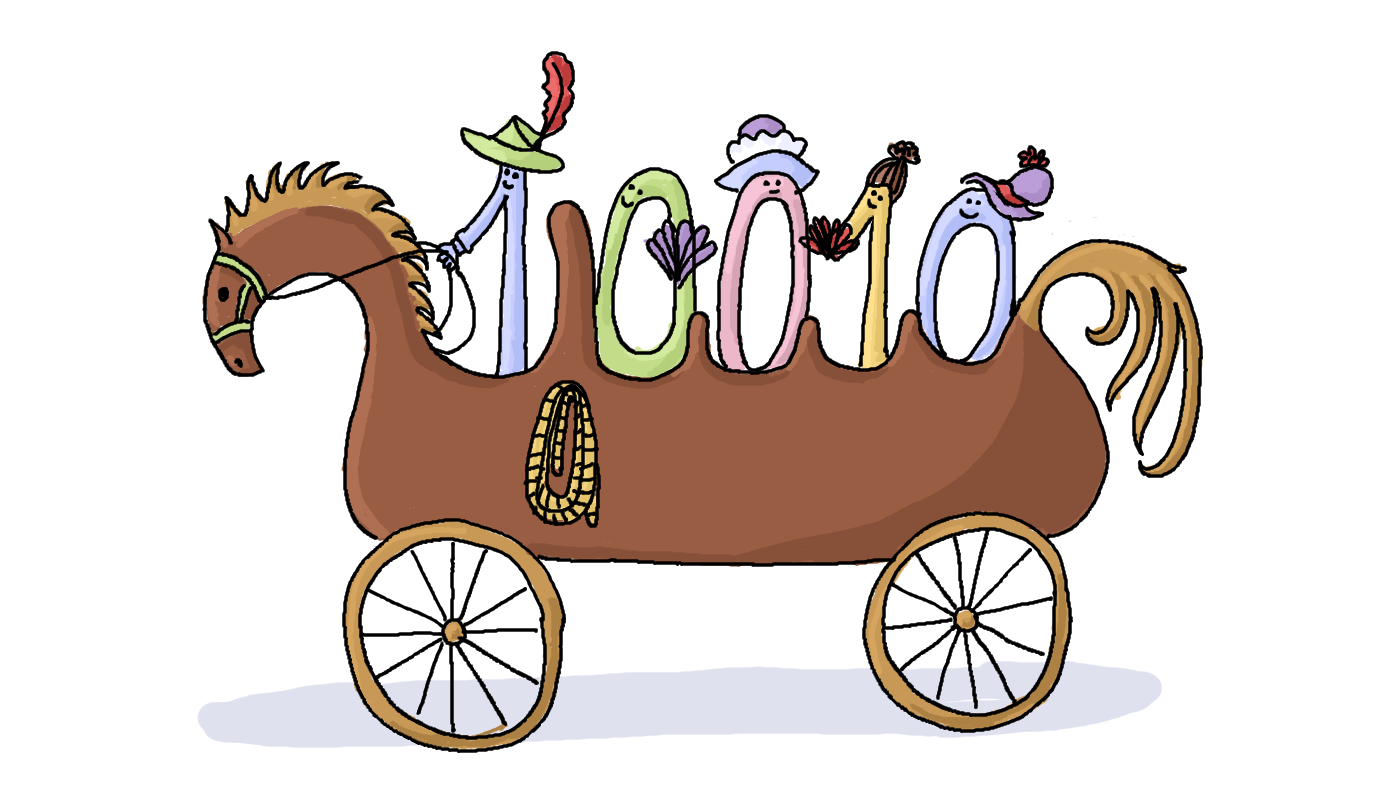
\includegraphics[width=\textwidth]{Pictures/Kutsche.png} 
\end{figure}

       Die SuS haben ausserdem in der vorherigen Stunde ein mechanisches Modell von Fliesskommazahlen gesehen, bestehend aus einem Holzkasten (Mantisse) mit einem Seil (Exponent).  Dieses Modell wird in dieser Stunde verwendet, um die Fliesskommazahlen besser kennenzulernen.
       Mit dem Kasten suchen die SuS die grösste und kleinste darstellbare Zahl, den Abstand zwischen benachbarten darstellbaren Zahlen und lernen, Fliesskommazahlen zu addieren. Bei der Addition sehen sie auch zwei Beispiele, wo das Ergebnis im Fliesskommazahlensystem mit der Intuition, die man aus den reellen Zahlen hat, nicht übereinstimmt.
Didaktische Varianten:
- Eiskapseln wie in Raumschiffe, um Zahlen einzufrieren, so dass sie weniger Platz bei der Transportierung brauchen. Damit sie wieder aufgetaut werden können, muss man wissen, wo man sie bezüglich dem Komma anpflanzen muss.
- Die Arche Noah. Die Zahlen werden von der grossen Flut gerettet. Für jede Zahl, die wir retten wollen, konstruieren wir so eine Arche. Aber es haben nicht alle Ziffern Platz. Welche nehmen wir ans Bord? Ziffern sind nicht alles, was wir brauchen, um die Zahl wieder zu rekonstruieren (dorthin zu bringen, wo sie war?). Wir brauchen auch das Seil mit dem Anker. Und natürlich werden solche Archen in einer Fabrik produziert, also haben wir mega viele davon, sind aber alle gleich (haben gleich viele Plätze und das Seil mit dem Anker ist gleich lang; das einzige, was wir ändern können, ist Anker umhängen). (Deswegen heissen sie ja Fliesskommazahlen).


\section*{Vorwissen}
       - sie können programmieren, aber das ist hier nicht wichtig
       - sie kennen Integers und Two’s Complement
       - sie kennen die Exponentialdarstellung (Chemie, Physik)
       - sie haben die Struktur (Vorzeichen, Mantisse, Exponent) von Fliesskommazahlen und die Metapher vom Kasten und Seil die Stunde davor gesehen
       Die LPU ist an SuS der Gymnasialstufe gerichtet. Das ist die zweite Stunde über Fliesskommazahlen. Ausserdem wissen die SuS schon, wie man Integer im Computer darstellt.
       Folgende Themen werden als Vorwissen angenommen und, wenn nötig, aufgefrischt:
       1. Exponentialdarstellung von Dezimalzahlen in Basis 10 (bekannt aus Chemie und Physik) Vorzeichen, Exponent, Mantisse, Basis
       2. Exponentialdarstellung von Dezimalzahlen in Basis 2, insbesondere ganze und rationale Zahlen in Binär umwandeln.

\section*{Lernziele}

\paragraph{Leitidee} Die SuS können nachvollziehen, wie der Computer “zaubert”.

\paragraph{Dispositionsziel} Die SuS vertrauen nicht mehr blind einem Computer bei Berechnungen mit reellen Zahlen.

\paragraph{Operationalisierte Lernziele}
\begin{itemize}
\item Die SuS finden die grösste und kleinste Zahl in einem Fliesskommazahlensystem.
\item Gegeben eine Fliesskommazahl, die SuS schreiben die nächste und die vorherige darstellbare Zahl auf.
\item Die SuS addieren zwei gegebene Fliesskommazahlen.
\end{itemize}




\end{document}
